%\part{title}% Source: http://tex.stackexchange.com/a/5374/23931
\documentclass[12pt]{article}
%\usepackage[turkish,english]{babel}
%\usepackage[T1]{fontenc}
\usepackage[utf8]{inputenc}
\usepackage[margin=1in]{geometry}
\usepackage[11pt]{moresize}
\usepackage{}

\usepackage{textcomp}

\usepackage[pdftex, bookmarksopen=true]{hyperref}
\usepackage[all]{hypcap}

\usepackage{amsmath}
\usepackage{mathtools}
\usepackage{listings}
\usepackage{tocbibind}
\usepackage{hyperref}
\usepackage{color}
\usepackage{textcomp}
\usepackage{geometry}
\usepackage{xcolor}
\usepackage{amsmath}
\usepackage[most]{tcolorbox}
\usepackage{amssymb}
\usepackage{pifont}
\usepackage{ulem}
\usepackage{cancel}
\usepackage{tikz}
\usepackage{fourier-orns}
\usepackage{longtable}
\usepackage{bm}
\usepackage{siunitx}
\usepackage{graphicx}

\usepackage{bookmark}

\usepackage{upgreek}
\usepackage[toc,page]{appendix}

\usepackage{mathtools}    % loads »amsmath«


\definecolor{mygreen}{RGB}{28,172,0} % color values Red, Green, Blue
\definecolor{mylilas}{RGB}{170,55,241}

\allowdisplaybreaks


\newcommand{\HRule}{\rule{\linewidth}{0.5mm}}
\newcommand{\Hrule}{\rule{\linewidth}{0.3mm}}

\DeclareMathOperator{\atantwo}{atan2}

\DeclarePairedDelimiter{\norm}{\lVert}{\rVert} 

\usepackage{xcolor}
\usepackage[linesnumbered,ruled,vlined]{algorithm2e}
\usepackage{algorithmic}
%%% Coloring the comment as blue
% comment style (algorithms)
\newcommand{\xCommentSty}[1]{\scriptsize\ttfamily\textcolor{blue}{#1}}
\SetCommentSty{xCommentSty}
%%%
\SetKwInput{KwInput}{Input}                % Set the Input
\SetKwInput{KwOutput}{Output}              % Set the Output
\SetKwInput{KwInitalize}{Initialize}       % set the Initialize

\DeclarePairedDelimiter\ceil{\lceil}{\rceil}
\DeclarePairedDelimiter\floor{\lfloor}{\rfloor}
\newcommand{\Mod}[1]{\ (\mathrm{mod}\ #1)}

\usepackage{subfig}

\newcommand{\nosemic}{\renewcommand{\@endalgocfline}{\relax}}% Drop semi-colon ;
\newcommand{\dosemic}{\renewcommand{\@endalgocfline}{\algocf@endline}}% Reinstate semi-colon ;
\newcommand{\pushline}{\Indp}% Indent
\newcommand{\popline}{\Indm\dosemic}% Undent
\let\oldnl\nl% Store \nl in \oldnl
\newcommand{\nonl}{\renewcommand{\nl}{\let\nl\oldnl}}% Remove line number for one line

\makeatletter% since there's an at-sign (@) in the command name
\renewcommand{\@maketitle}{%
	\parindent=0pt% don't indent paragraphs in the title block
	\centering
	{\Large \bfseries\textsc{\@title}}
	\HRule\par%
	\textit{\@author \hfill \@date}
	\par
}
\makeatother% resets the meaning of the at-sign (@)

\setcounter{MaxMatrixCols}{20}

\newcommand*{\doi}[1]{\href{http://dx.doi.org/#1}{doi: #1}}

\title{Demonstration: Oscillating Masses For Linear-MPC Benchmarks}
\author{İ. Ç. Yılmaz}
\date{\today}

\renewcommand\refname{References}

\lstset{language=Matlab,%
	%basicstyle=\color{red},
	breaklines=true,%
	morekeywords={matlab2tikz},
	keywordstyle=\color{blue},%
	morekeywords=[2]{1}, keywordstyle=[2]{\color{black}},
	identifierstyle=\color{black},%
	stringstyle=\color{mylilas},
	commentstyle=\color{mygreen},%
	showstringspaces=false,%without this there will be a symbol in the places where there is a space
	numbers=left,%
	numberstyle={\tiny \color{black}},% size of the numbers
	numbersep=9pt, % this defines how far the numbers are from the text
	emph=[1]{for,end,break},emphstyle=[1]\color{red}, %some words to emphasise
	%emph=[2]{word1,word2}, emphstyle=[2]{style},  
}

\makeatletter
\setlength{\@fptop}{0pt}
\makeatother

\begin{document}
\maketitle% prints the title block
\begin{figure}[b]
	\centering
	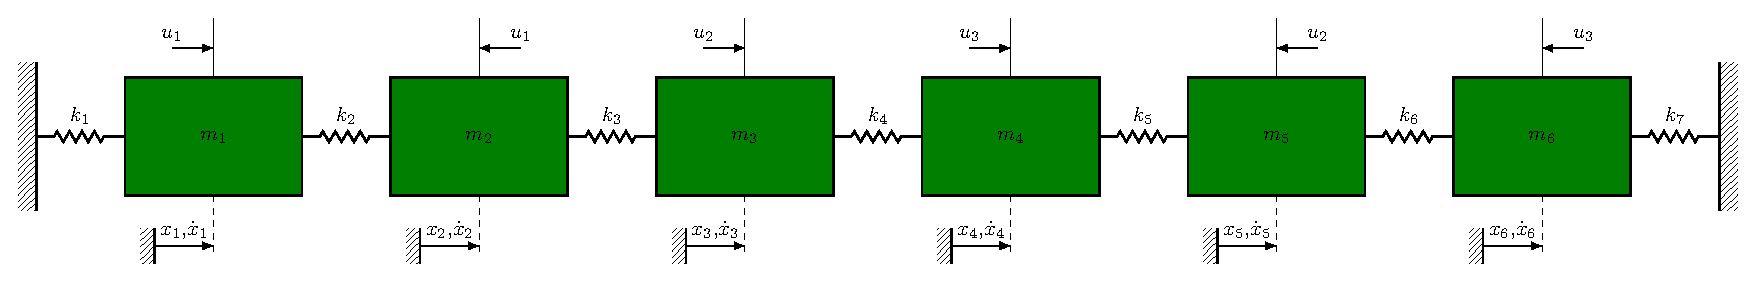
\includegraphics[width=1.0\textwidth,keepaspectratio]{images/oscillating_masses_tikz.pdf}
	\caption{The model of oscillating masses.} 
	\label{fig:oscillating_masses}	
\end{figure}
\section{Mathematical Modeling} \label{Mathematical_Modeling}
\noindent This demonstration consists of a sequence of six masses connected by springs to each other, and to walls on either side, as shown in Fig. \ref{fig:oscillating_masses}. There are three actuators, $u_{1}$, $u_{2}$, $u_{3}$ , which exert tensions between different masses. The masses, $m_{1}$, $m_{2}$, $m_{3}$, $m_{4}$, $m_{5}$, $m_{6}$, have value $1$ kg, the springs
all have spring constant $1$ $kg/s^{2}$, and there is no damping \cite{Wang2010}. \newline
\par\noindent Continuous time system can be sampled by using a first order
hold model, with a period of 0.5 (which is around 3 times faster than the period of the fastest oscillatory mode of the open-loop
system). The state vector is $\bm{x} = [x_{1}\,\,x_{2}\,\,x_{3}\,\,x_{4}\,\,x_{5}\,\,x_{6}\,\,\dot{x}_{1}\,\,\dot{x}_{2}\,\,\dot{x}_{3}\,\,\dot{x}_{4}\,\,\dot{x}_{5}\,\,\dot{x}_{6}]^T$ where $x_{i}$ is the position of mass $i$ while $\dot{x}_{i}$ is the velocity of mass $i$ on the horizontal axis. Dynamic equations for all masses with inputs of the system can be written as
\begin{subequations} 
	\label{eqn:dynamical_equations}
	\begin{align} 
		m_{1}\ddot{x}_{1} &= u_{1} - k_{1}x_{1} + k_{2}(x_{2}-x_{1}) \\ 
		\ddot{x}_{1} &= \frac{1}{m_{1}}u_{1} - \frac{k_{1}+k_{2}}{m_{1}}x_{1} + \frac{k_{2}}{m_{1}}x_{2} \nonumber \\ 
		m_{2}\ddot{x}_{2} &= -u_{1} - k_{2}(x_{2}-x_{1}) + k_{3}(x_{3}-x_{2}) \\ 
		\ddot{x}_{2} &= -\frac{1}{m_{2}}u_{1} + \frac{k_{2}}{m_{2}}x_{1} -   \frac{k_{2}+k_{3}}{m_{2}}x_{2} + \frac{k_{3}}{m_{2}}x_{3} \nonumber \\
		m_{3}\ddot{x}_{3} &= u_{2} - k_{3}(x_{3}-x_{2}) + k_{4}(x_{4}-x_{3}) \\ 
		\ddot{x}_{3} &= \frac{1}{m_{3}}u_{2} + \frac{k_{3}}{m_{3}}x_{2} -   \frac{k_{3}+k_{4}}{m_{3}}x_{2} + \frac{k_{4}}{m_{3}}x_{4} \nonumber \\	
		m_{4}\ddot{x}_{4} &= u_{3} - k_{4}(x_{4}-x_{3}) + k_{5}(x_{5}-x_{4}) \\ 
		\ddot{x}_{4} &= \frac{1}{m_{4}}u_{3} + \frac{k_{4}}{m_{4}}x_{3} -   \frac{k_{4}+k_{5}}{m_{4}}x_{4} + \frac{k_{5}}{m_{4}}x_{5} \nonumber \\
		m_{5}\ddot{x}_{5} &= -u_{2} - k_{5}(x_{5}-x_{4}) + k_{6}(x_{6}-x_{5}) \\ 
		\ddot{x}_{5} &= -\frac{1}{m_{5}}u_{2} + \frac{k_{5}}{m_{5}}x_{4} -   \frac{k_{5}+k_{6}}{m_{5}}x_{4} + \frac{k_{6}}{m_{5}}x_{6} \nonumber \\	 		
		m_{6}\ddot{x}_{6} &= -u_{3} - k_{6}(x_{6}-x_{5}) - k_{7}x_{6} \\ 
		\ddot{x}_{6} &= -\frac{1}{m_{6}}u_{3} + \frac{k_{6}}{m_{6}}x_{5} -   \frac{k_{6}+k_{7}}{m_{6}}x_{6} \nonumber 
	\end{align} 
\end{subequations}
\par\noindent The state space representation of the oscillation interconnected masses can be written in matrix form as follows:  
\begin{align}
	\label{eqn:discrete_state_space_matrix_form}
	\bm{\dot{x}}(t) &= \underbrace{\begin{bmatrix}
			0 & 0 & 0 & 0 & 0 & 0 & 1 & 0 & 0 & 0 & 0 & 0 \\    
			0 & 0 & 0 & 0 & 0 & 0 & 0 & 1 & 0 & 0 & 0 & 0 \\
			0 & 0 & 0 & 0 & 0 & 0 & 0 & 0 & 1 & 0 & 0 & 0 \\
			0 & 0 & 0 & 0 & 0 & 0 & 0 & 0 & 0 & 1 & 0 & 0 \\
			0 & 0 & 0 & 0 & 0 & 0 & 0 & 0 & 0 & 0 & 1 & 0 \\
			0 & 0 & 0 & 0 & 0 & 0 & 0 & 0 & 0 & 0 & 0 & 1 \\
			-\frac{k_{1}+k_{2}}{m_{1}} & \frac{k_{2}}{m_{1}} & 0 & 0 & 0 & 0 & 0 & 0 & 0 & 0 & 0 & 0 \\
			\frac{k_{2}}{m_{2}} & -\frac{k_{2}+k_{3}}{m_{2}} & \frac{k_{3}}{m_{2}} & 0 & 0 & 0 & 0 & 0 & 0 & 0 & 0 & 0 \\
			0 & \frac{k_{3}}{m_{3}} & -\frac{k_{3}+k_{4}}{m_{3}} & \frac{k_{4}}{m_{3}} & 0 & 0 & 0 & 0 & 0 & 0 & 0 & 0 \\
			0 & 0 & \frac{k_{4}}{m_{4}} & -\frac{k_{4}+k_{5}}{m_{4}} & \frac{k_{5}}{m_{4}} & 0 & 0 & 0 & 0 & 0 & 0 & 0 \\
			0 & 0 & 0 & \frac{k_{5}}{m_{5}} & -\frac{k_{5}+k_{6}}{m_{5}} & \frac{k_{6}}{m_{5}} & 0 & 0 & 0 & 0 & 0 & 0 \\
			0 & 0 & 0 & 0 & \frac{k_{6}}{m_{6}} & -\frac{k_{6}+k_{7}}{m_{6}} & 0 & 0 & 0 & 0 & 0 & 0 \nonumber \\
	\end{bmatrix}}_{\let\scriptstyle\textstyle\substack{\bm{A}_{c}}} \bm{x}(t) \\ &+ \underbrace{\begin{bmatrix}
			0 & 0 & 0 \\
			0 & 0 & 0 \\
			0 & 0 & 0 \\
			0 & 0 & 0 \\
			0 & 0 & 0 \\
			0 & 0 & 0 \\
			\frac{1}{m_{1}} & 0 & 0 \\
			-\frac{1}{m_{2}} & 0 & 0 \\
			0 & \frac{1}{m_{3}} & 0 \\
			0 & 0 & \frac{1}{m_{4}} \\
			0 & -\frac{1}{m_{5}} & 0 \\
			0 & 0 & \frac{1}{m_{6}} \\
	\end{bmatrix}}_{\let\scriptstyle\textstyle\substack{\bm{B}_{c}}}\bm{u}(t)	
\end{align}
\par \noindent All dynamic equations are in the form of $\bm{\dot{x}}(t)=\bm{A}_{c}\bm{x}(t)\,+\,\bm{B}_{c}u(t)$. If the state equations $\dot{\bm{x}}(t) = \bm{A}_{c}\bm{x}(t)\,+\,\bm{B}_{c}u(t)$ are rearranged, and all terms pre-multiplied by the square matrix $e^{-\bm{A}_{c}t}$:
\begin{equation}
	\label{eqn:Solution_of_state_space equation_1}
	e^{-\bm{A}_{c}t}\dot{\bm{x}}(t) - e^{-\bm{A}_{c}t}\bm{A}\bm{x}(t) = \frac{d}{dt}\bigg(e^{-\bm{A}_{c}t}\bm{x}(t)\bigg)  = e^{-\bm{A}_{c}t}\bm{B}_{c}u(t)
\end{equation}
\noindent Integration of Eq. \ref{eqn:Solution_of_state_space equation_1} gives
\begin{equation}
	\label{eqn:Solution_of_state_space equation_2}
	\int_{0}^{t}\frac{d}{d\tau}\bigg(e^{-\bm{A}_{c}\tau}\bm{x}(\tau)\bigg) d\tau = \int_{0}^{t} e^{-\bm{A}_{c}t}\bm{B}_{c}u(t) =  e^{-\bm{A}_{c}t}\bm{x}(t) - e^{-\bm{A}_{c}0}\bm{x}(0) = \int_{0}^{t} e^{-\bm{A}_{c}\tau}\bm{B}_{c}u(\tau)d\tau
\end{equation}
\noindent where $e^{-\bm{A}_{c}0} = \bm{I}$ is $12\times12$ identity matrix and $[e^{-\bm{A}_{c}t}]^{-1} = e^{\bm{A}t}$ the complete state vector response may be written in two similar forms
\begin{subequations} 
	\label{eqn:Solution_of_state_space equation_3}
	\begin{align} 
		\bm{x}(t) &= e^{\bm{A}_{c}t}\bm{x}(0)  + e^{\bm{A}_{c}t}\int_{0}^{t} e^{-\bm{A}_{c}\tau}\bm{B}_{c}u(\tau)d\tau\\
		\bm{x}(t) &= e^{\bm{A}_{c}t}\bm{x}(0)  + \int_{0}^{t} e^{\bm{A}_{c}(t-\tau)}\bm{B}_{c}u(\tau)d\tau
	\end{align} 
\end{subequations}
\noindent A continuous time signal $\{x(t)\}$ can be obtained from a discrete time (DT) signal ${x[k]}$, by holding the value of the DT signal constant for one sampling period $T$ or $\Delta t$, such that: This is known as the \text{zero-order hold}. The discrete-time equivalent of continuous time equation is of the form:
\begin{align}
	\begin{split}
		\bm{x}[k+1] &= \bm{A_{d}}\bm{x}[k] + \bm{B_{d}}u[k] \\
	\end{split}
\end{align}
\noindent Starting from the solution of the continuous state-space equation \ref{eqn:Solution_of_state_space equation_3}, that the corresponding discrete matrices are obtained as: 
\begin{equation}
	\label{eqn:discrete_system_matrices}
	\bm{A_d} = e^{\bm{A}_{c}T}\;\;\;\text{and}\;\;\;\bm{B_{d}}=\bigg(\int_{0}^{T}e^{\bm{A}_{c}\tau}d\tau\bigg)\bm{B}_{c} = \bm{A}_{c}^{-1}(e^{\bm{A}_{c}T}-\bm{I})\bm{B}_{c} 
\end{equation}
\noindent It should be note that that this is the \textit{exact} solution to the differential equation, there are no discretization errors. While it is exact, information is still lost by the discretization: the inter-sample behavior.

\lstinputlisting{MATLAB_File/model_and_discretization.m} 

\section{MPC Formulation and Some Solvers In the Literature} \label{MPC_Formulation}
In order to evaluate the performance of the solver for various problem sizes, the following MPC problem is formulated for a chain of masses interconnected with spring-dampers \cite{Domahidi2012}:

\begin{equation}
	\begin{aligned}
		\min_{\bm{U}} V_{n}(\bm{x},\bm{U})  & := \sum_{k=k_{0}}^{k_{0}+N-1} \bm{x}_{k}^{T}\bm{Q}\bm{x}_{k} + \bm{u}_{k}^{T}\bm{R}\bm{u}_{k} + V_{f}(\bm{x}_{k_{0}+N})\\
		\textrm{s.t.} \quad & \bm{x}_{k_{0}} = \bm{x}(k_{0}),\\
	    & \bm{x}_{k+1} = \bm{A}_{k}\bm{x}_{k} + \bm{B}_{k}\bm{u}_{k}  &&k_{0} \leq k < k_{0} + N, \\
	    & -4\bm{\cdot}\bm{1}_{n_x} \leq \bm{x}_{k} \leq 4\bm{\cdot}\bm{1}_{n_x}  &&k_{0} \leq k \leq k_{0} + N,\\
	    & -0.5\bm{\cdot}\bm{1}_{n_u} \leq \bm{u}_{k} \leq 0.5\bm{\cdot}\bm{1}_{n_u}  &&k_{0} \leq k < k_{0} + N.
	\end{aligned}
\end{equation}
with $V_{f}(k_{0}+N) := \bm{x}_{k_{0}+N}^{T}\bm{Q}\bm{x}_{k_{0}+N}$.  Note
that this formulation does not provide stability guarantees since no terminal constraint is included. \newline 

\par \noindent For this optimization problem, dozen of academic works have been done. Wang and Body utilizes the above optimization problem via block-wise Cholesky factorization \cite{Wang2010}. In addition to the method that have been employed in \cite{Wang2010}, rank one modifications in the computation is defined in the \cite{Domahidi2012}. Solution time of the problem, especially in the large horizon size and state variables size is improved. \newline

\par \noindent Frison \textit{et. al.}, \cite{Frison2018}, selects linear chain of masses springs problem by using Dual-Newton strategy for QP problem. In this study main aim is to show demonstration how the linear algebra provided in BLASFEO (Basic Linear Algebra Subroutines for Emdedded Optimization) can enhance the performance of new or existing embedded optimization tools. The results indicate that using BLASFEO
throughout the code can lead to significant performance gains. With BLASFEO Library, a HPIPM (High Performance Interior Point Method) framework have been developed for linear model predictive control. Same problem has also been employed in this study \cite{Frison2020}. Three types of QP are taken into consideration and some implementation choices, $\mid$\textbf{speed\_abs}$\mid$\textbf{speed}$\mid$\textbf{balance}$\mid$ \textbf{robust}$\mid$, are given as mode in the solver.   
 


\clearpage
\bibliographystyle{plainurl}
\bibliography{references}
% You can use full name of authors, however most likely some of the Bibtex entries you will find, will use abbreviated first names
% If you don't want to correct each of them by hand, you can use abbreviated style for all of the references
\clearpage

\end{document}

